\chapter{A visual route through the consolidated core}
These eight vector figures were generated by the original Python programs. Each remains associated with its source volume and caption. Curves at finite parameters are illustrations or bounded numerical evidence; the mathematical conclusions and their qualifications are stated in Chapters 1--3.
\clearpage
\section*{1. Exact coefficient packets}
\addcontentsline{toc}{section}{1. Exact coefficient packets}
\begin{figure}[H]
\centering
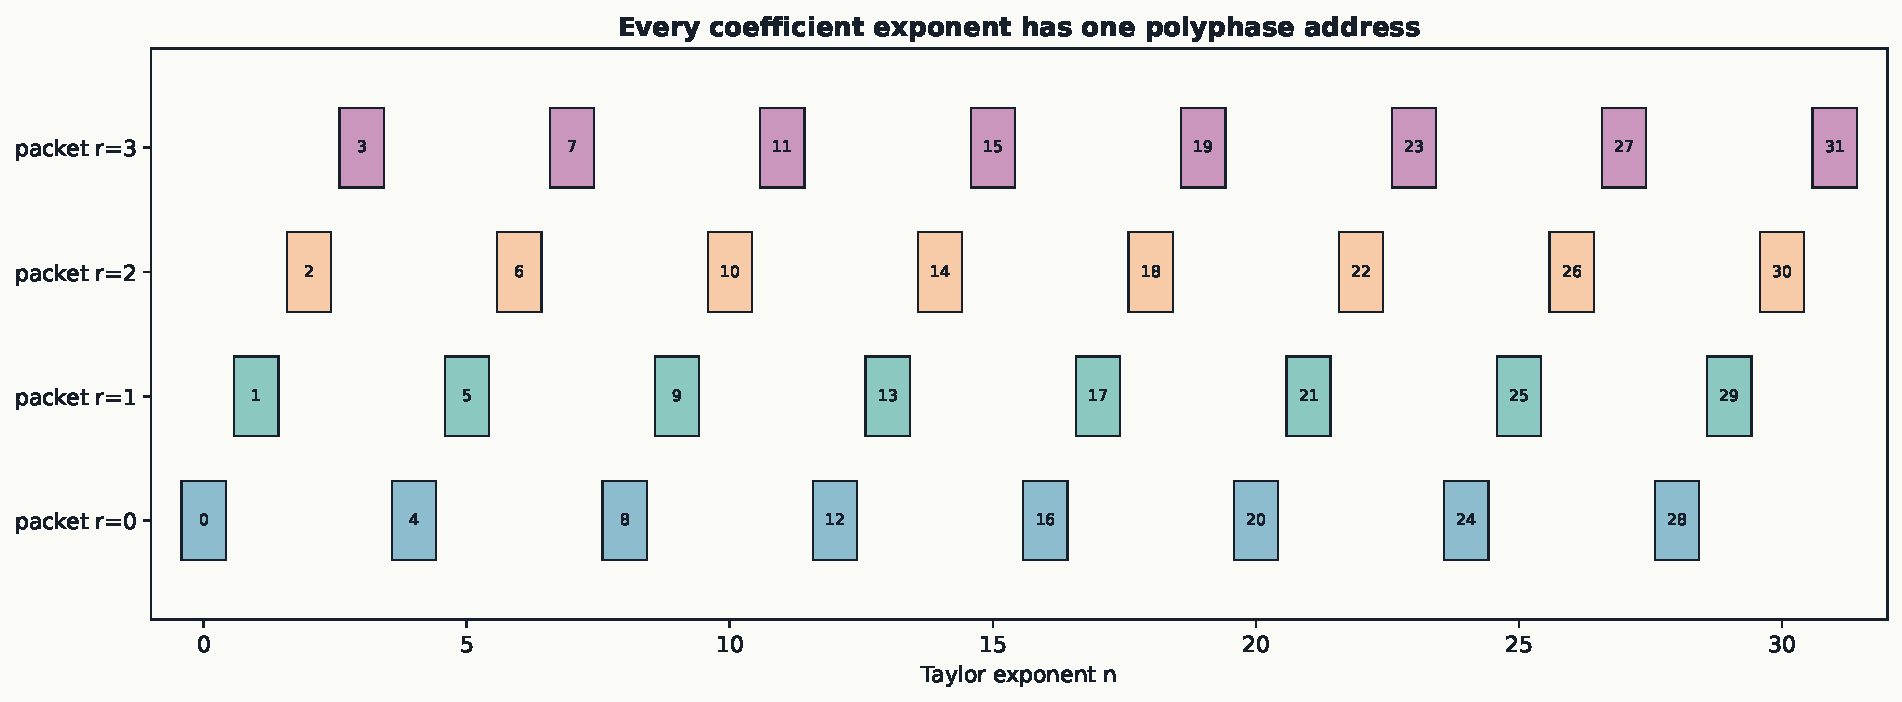
\includegraphics[width=\textwidth,height=0.60\textheight,keepaspectratio]{figures/I_01_polyphase_partition.pdf}
\caption{Residue addresses partition the coefficients and retain exact reconstruction. This is the algebraic entry point of Chapter 1. Source: Volume I, figure 01.}
\end{figure}
\clearpage
\section*{2. The arithmetic Gamma scale}
\addcontentsline{toc}{section}{2. The arithmetic Gamma scale}
\begin{figure}[H]
\centering
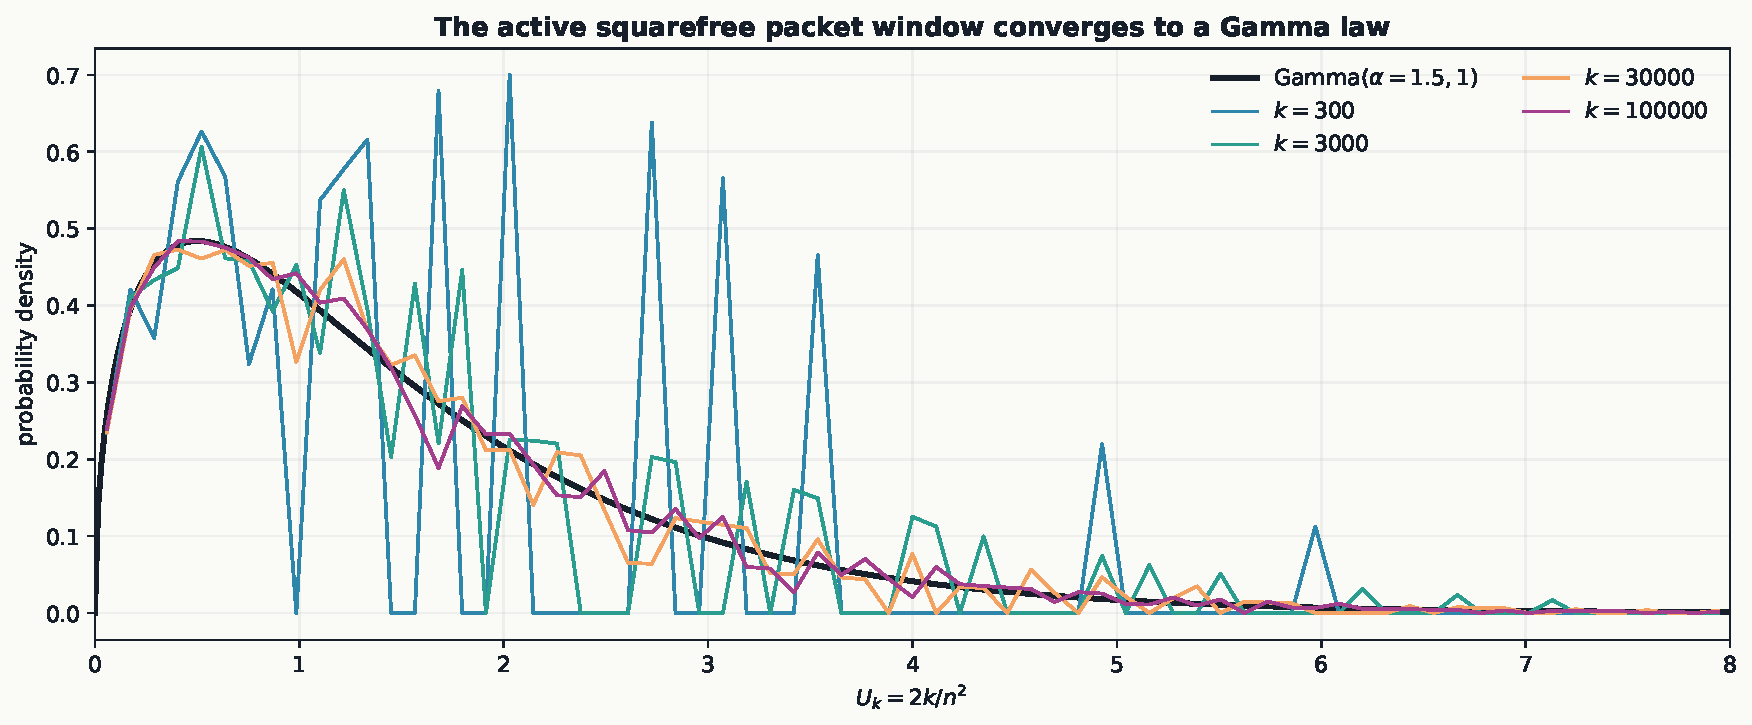
\includegraphics[width=\textwidth,height=0.60\textheight,keepaspectratio]{figures/II_14_gamma_scaling.pdf}
\caption{The finite-depth distributions approach the Gamma coordinate law. Chapter 1 separates the visual evidence from the all-moment proof. Source: Volume II, figure 14.}
\end{figure}
\clearpage
\section*{3. A common Laguerre fixed point}
\addcontentsline{toc}{section}{3. A common Laguerre fixed point}
\begin{figure}[H]
\centering
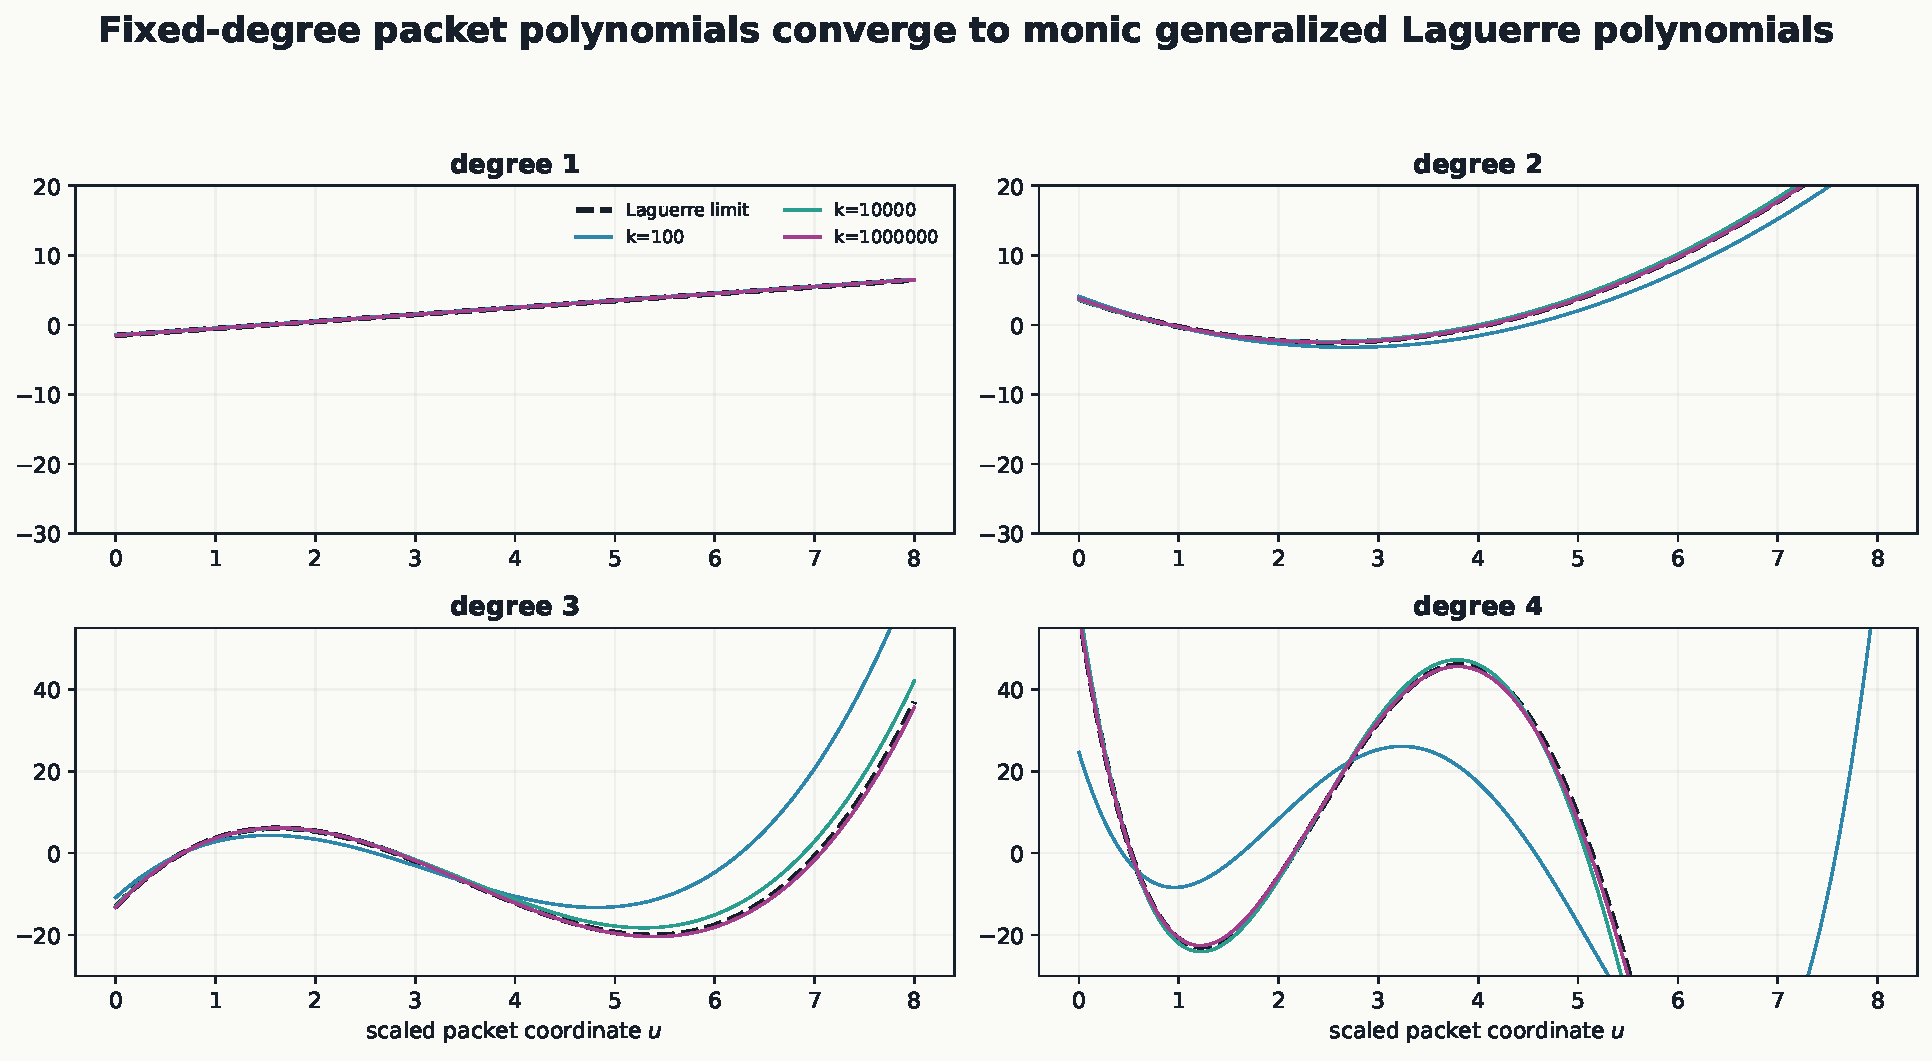
\includegraphics[width=\textwidth,height=0.60\textheight,keepaspectratio]{figures/III_13_laguerre_polynomial_limit.pdf}
\caption{Fixed-degree orthogonal polynomials converge after endpoint rescaling. The limiting moment matrix supplies the coefficient argument. Source: Volume III, figure 13.}
\end{figure}
\clearpage
\section*{4. The exact Gamma--sech window}
\addcontentsline{toc}{section}{4. The exact Gamma--sech window}
\begin{figure}[H]
\centering
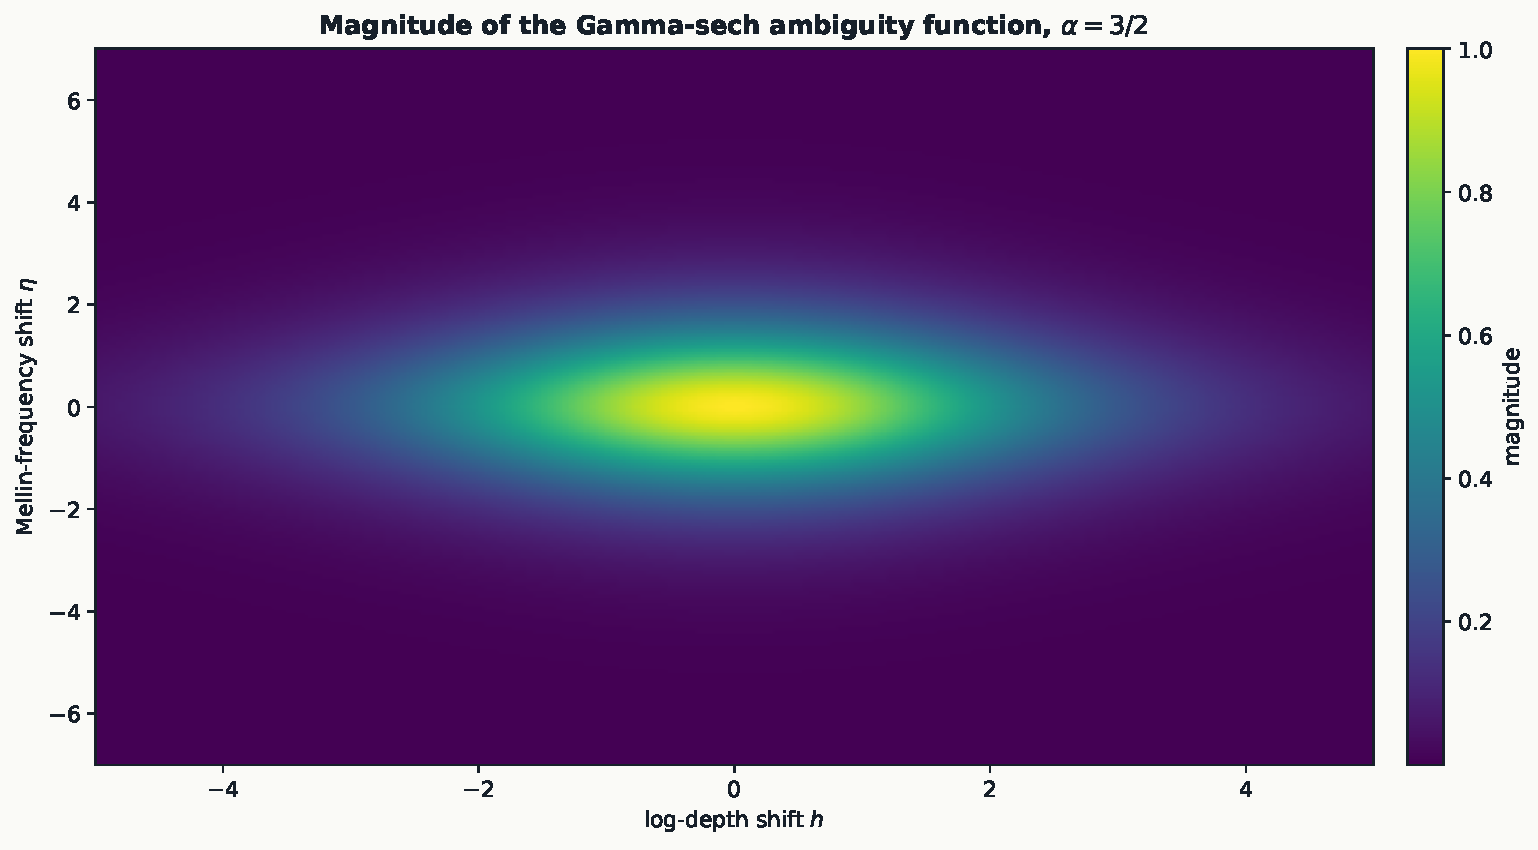
\includegraphics[width=\textwidth,height=0.60\textheight,keepaspectratio]{figures/V_06_ambiguity_magnitude.pdf}
\caption{The phase-space magnitude is generated from the normalized log-Gamma window. The corresponding cross-shape formula is proved in Chapter 2. Source: Volume V, figure 06.}
\end{figure}
\clearpage
\section*{5. Shape refinement}
\addcontentsline{toc}{section}{5. Shape refinement}
\begin{figure}[H]
\centering
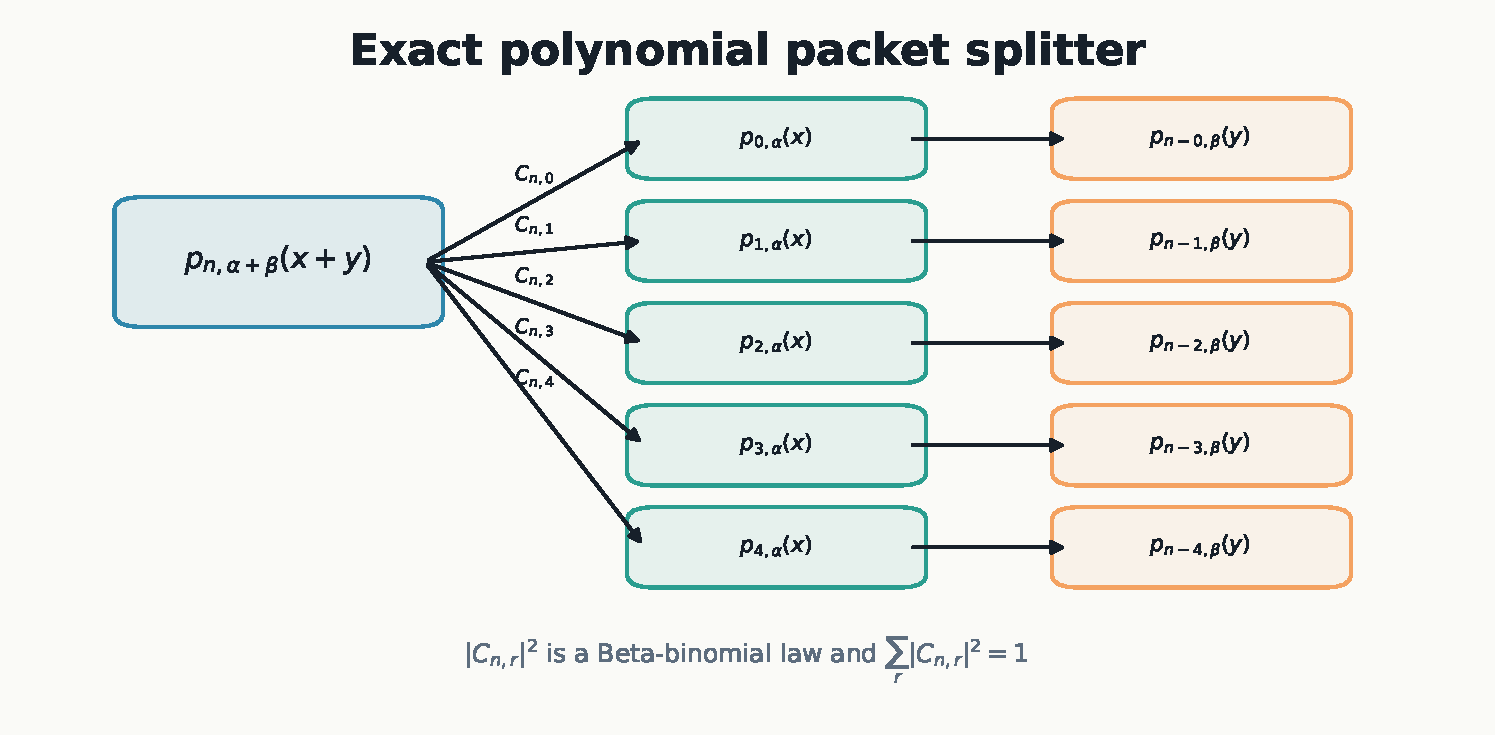
\includegraphics[width=\textwidth,height=0.60\textheight,keepaspectratio]{figures/VI_12_packet_splitter.pdf}
\caption{The normalized polynomial refinement distributes one total degree across two child shapes. Its squared coefficients form a beta-binomial law. Source: Volume VI, figure 12.}
\end{figure}
\clearpage
\section*{6. Finite recoupling}
\addcontentsline{toc}{section}{6. Finite recoupling}
\begin{figure}[H]
\centering
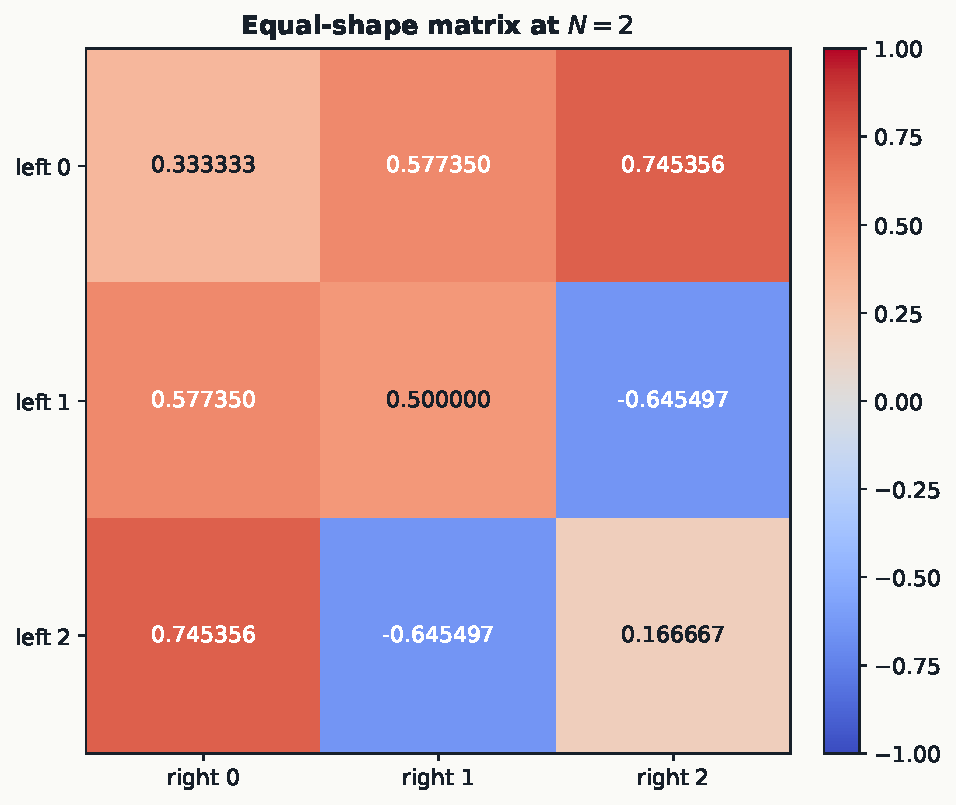
\includegraphics[width=\textwidth,height=0.60\textheight,keepaspectratio]{figures/VII_08_two_excitation_exact.pdf}
\caption{Signed amplitudes and their squared probabilities are different outputs of one finite transform. The gauge affects amplitude signs while preserving the measured kernel. Source: Volume VII, figure 08.}
\end{figure}
\clearpage
\section*{7. A deformable two-channel packet}
\addcontentsline{toc}{section}{7. A deformable two-channel packet}
\begin{figure}[H]
\centering
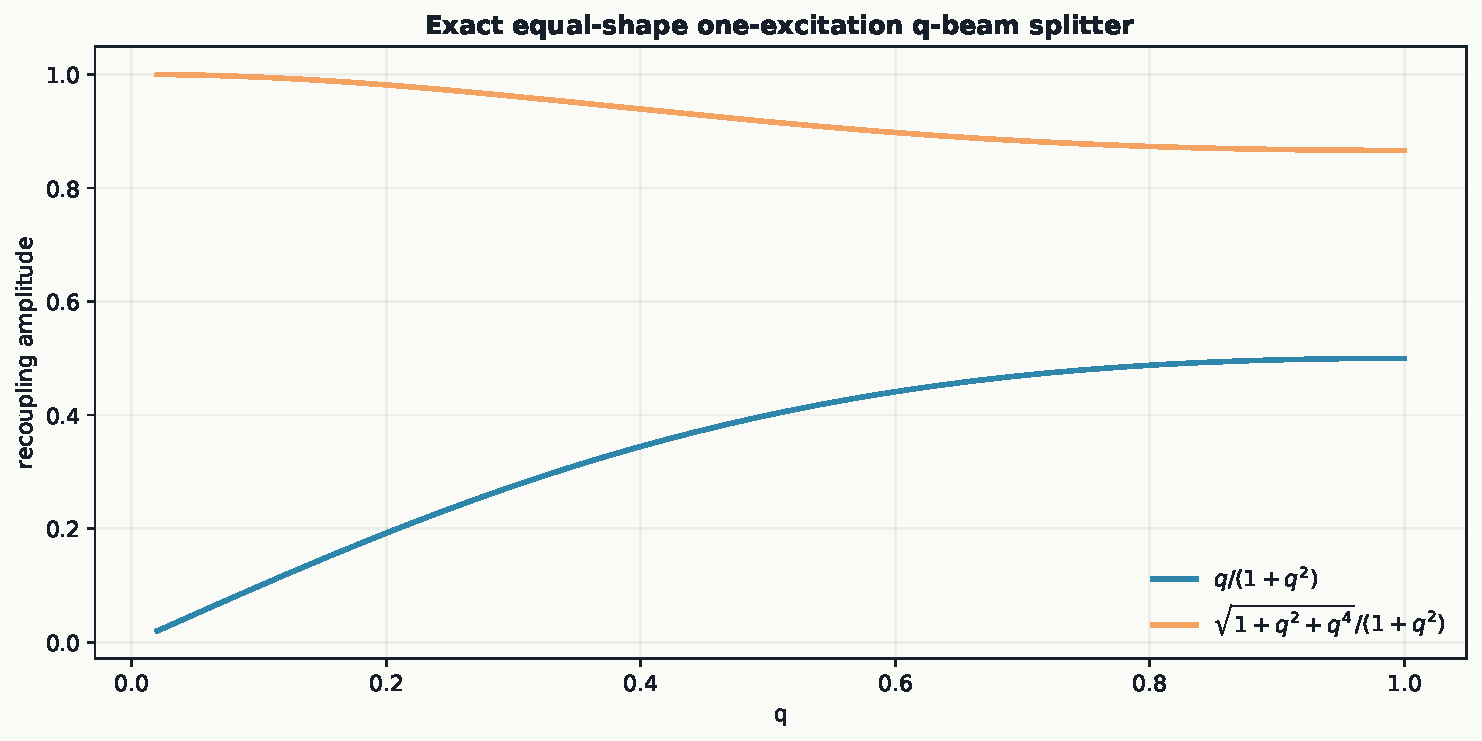
\includegraphics[width=\textwidth,height=0.60\textheight,keepaspectratio]{figures/VIII_07_q_beam_splitter_amplitudes.pdf}
\caption{The exactly derived one-excitation overlap connects classical mixing with a sparse routing limit. Higher-degree behavior requires its own analysis. Source: Volume VIII, figure 07.}
\end{figure}
\clearpage
\section*{8. A retained negative control}
\addcontentsline{toc}{section}{8. A retained negative control}
\begin{figure}[H]
\centering
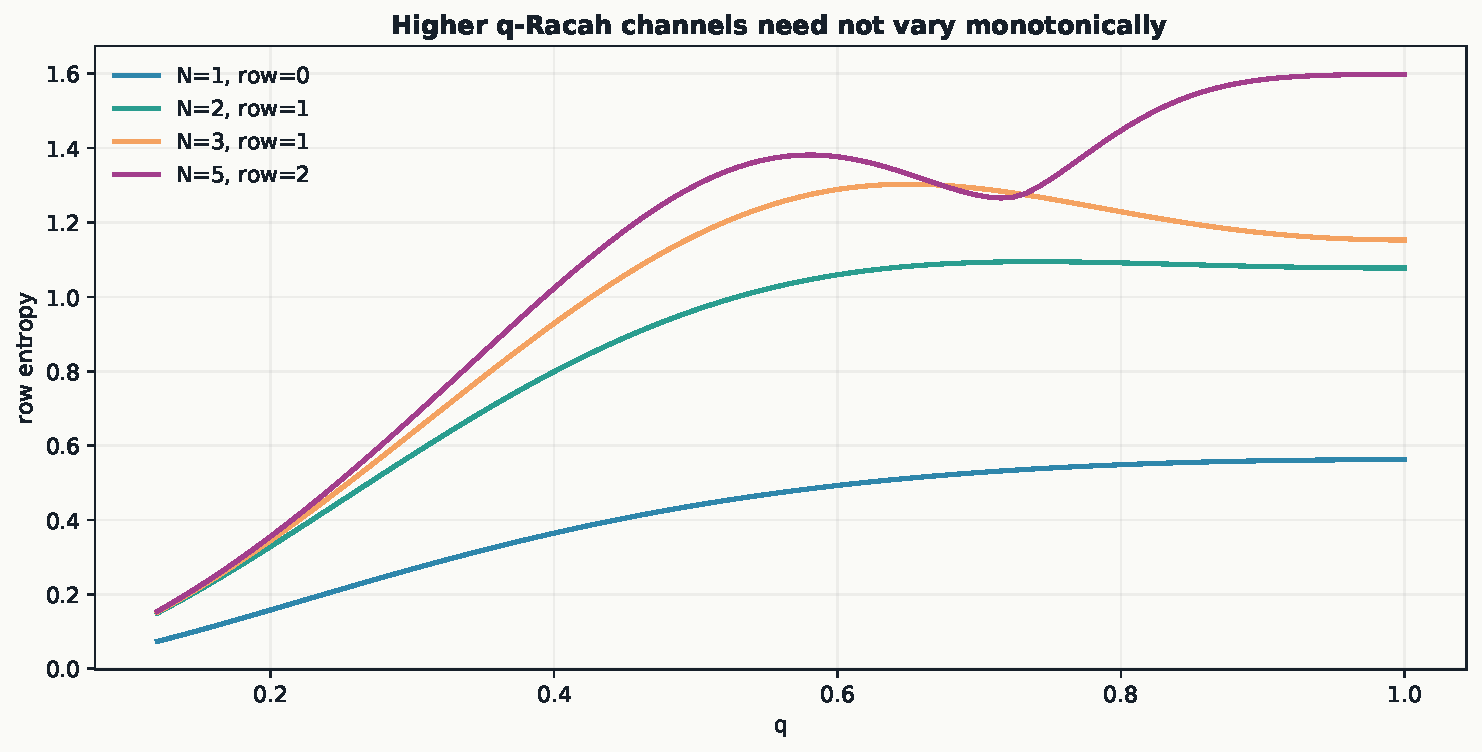
\includegraphics[width=\textwidth,height=0.60\textheight,keepaspectratio]{figures/VIII_21_entropy_nonmonotonicity.pdf}
\caption{The source figure exhibits a higher-excitation entropy decrement as q varies. Fixed-kernel entropy nondecrease after measurement does not imply monotonicity along deformation. Source: Volume VIII, figure 21.}
\end{figure}
